\documentclass[11pt]{article}
\usepackage[a4paper,margin=1in]{geometry}
\usepackage{fontspec}
\usepackage{graphicx}
\usepackage{booktabs}
\usepackage{hyperref}
\usepackage{enumitem}
\usepackage{float}
\usepackage{setspace}

\setmainfont{Noto Sans CJK KR}
\setlength{\parskip}{0.5em}
\setlength{\parindent}{0pt}
\tolerance=1000
\emergencystretch=3em
\hfuzz=2pt
\sloppy
\onehalfspacing

\title{Selective Refinement Status Report\\Revised Summary for 2026-04-09}
\author{}
\date{}

\begin{document}
\maketitle

\section{Executive Summary}

이번 라운드에서 살아남은 것은 \texttt{two\_pass} 하나뿐이다. 그러나 현재 checked revision의
\texttt{exp\_query\_exploit.py}와 \texttt{exp\_cliffkv\_niah.py}는 둘 다 FP16 underlying cache를 유지한 채
attention path만 바꾼다. 따라서 지금까지의 positive result는 storage-valid compression evidence가 아니라
attention-path diagnostic evidence다.

현재까지 확인된 핵심 수치는 다음과 같다. earlier remote run의 Mistral 4K same-harness에서
\texttt{baseline\_2bit = 0.333}, \texttt{two\_pass\_k16 = 1.000},
\texttt{query\_dequant} 최고값은 \texttt{0.333}, \texttt{sharp\_temp}는 \texttt{0.000}이었다.
Qwen 4K에서도 \texttt{two\_pass\_k8/k16/k32/k64}가 모두 \texttt{1.000}이었다.
반면 QDRP는 real-trace story가 약하고, TRIC는 synthetic에서도 shared linear baseline을 넘지 못했다.

다만 current checked revision의 fresh local bounded rerun은 이 positive result를 그대로 재현하지 못했다.
Mistral 4K, depths \{0.1, 0.5, 0.9\}, \texttt{repeats=1}에서
\texttt{two\_pass\_k8 = 0.000}, \texttt{two\_pass\_k16 = 0.000}이었다.
지금은 method claim보다 reproducibility audit이 먼저다.

\section{Verified Facts}

\begin{table}[H]
\centering
\small
\begin{tabular}{p{0.43\linewidth}p{0.14\linewidth}p{0.31\linewidth}}
\toprule
Fact & Value & Source \\
\midrule
Mistral 4K \texttt{baseline\_2bit} & \texttt{0.333} & \texttt{mistral\_all\_methods\_4k.json} \\
Mistral 4K \texttt{two\_pass\_k16} & \texttt{1.000} & \texttt{mistral\_all\_methods\_4k.json} \\
Best Mistral 4K \texttt{query\_dequant} & \texttt{0.333} & \texttt{mistral\_all\_methods\_4k.json} \\
Best Mistral 4K \texttt{sharp\_temp} & \texttt{0.000} & \texttt{mistral\_all\_methods\_4k.json} \\
Mistral 4K \texttt{two\_pass\_k8/k16/k32/k64} & all \texttt{1.000} & \texttt{mistral\_two\_pass\_4k.json} \\
Qwen 4K \texttt{two\_pass\_k8/k16/k32/k64} & all \texttt{1.000} & \texttt{qwen\_two\_pass\_4k.json} \\
QDRP low-budget synthetic & \texttt{+0.3770} & \texttt{autoresearch\_dynamic\_recursive\_log.tsv} \\
QDRP budget=2 pure risk & \texttt{-0.1240} & \texttt{autoresearch\_dynamic\_recursive\_log.tsv} \\
TRIC \texttt{recursive\_gain\_vs\_linear} & negative in all logged runs & \texttt{autoresearch\_dynamic\_recursive\_log.tsv} \\
Fresh local rerun \texttt{two\_pass\_k8/k16} & both \texttt{0.000} & \texttt{results/query\_exploit\_validity} \\
\bottomrule
\end{tabular}
\end{table}

\section{What The Current Results Actually Mean}

\subsection{Two-Pass Survived, But Only As A Diagnostic}

\texttt{two\_pass} clearly beat the bounded 2-bit baseline in the earlier remote harness,
but the current checked revision did not reproduce that win in a fresh local bounded rerun.
That makes it worth keeping only as a diagnostic candidate. It does not yet make it a
compression method, because the stored cache itself is still not replaced by a true
low-bit representation.

\subsection{Query Dequantization And Temperature Sharpening Failed}

The same-harness comparison is already decisive enough to narrow the wave.
\texttt{query\_dequant} never beat the baseline on the 4K bounded run, and
\texttt{sharp\_temp} failed at every tested temperature. These ideas should not receive
more GPU time until a more direct score-level diagnostic gives them new footing.

\subsection{QDRP And TRIC Are Below The Bar}

QDRP only helps in the synthetic \texttt{budget=1} toy regime. At \texttt{budget=2},
pure risk selection collapses and hybrid becomes essentially tied with score selection.
TRIC is worse: it still loses to a shared linear baseline, so there is no current reason
to spend end-to-end GPU budget on it.

\section{Open Failure Modes}

\begin{itemize}[leftmargin=1.5em]
\item Recency artifact: \texttt{two\_pass} may be selecting near-query tokens rather than the true needle region.
\item Attention sink artifact: early sink tokens may be enough to flip binary NIAH.
\item Selection-repair coupling: selection and repair happen inside the same wrapper.
\item Saturated 4K binary NIAH: \texttt{k=8} already saturates, so this grid cannot reveal the true frontier.
\item Budget ambiguity: current average-bit numbers are upper-bound access proxies, not stored-cache budgets.
\end{itemize}

\section{Next Plan}

The next step order is strict.

\begin{enumerate}[leftmargin=1.5em]
\item Audit the reproduction gap between the earlier remote win and the current checked revision.
\item Run \texttt{two\_pass} against \texttt{recent\_k}, \texttt{sink\_k}, and \texttt{random\_k} controls.
\item Only if reproduction is stable, move to 8K/16K with \texttt{k=1,2,4,8,16}.
\item Implement true storage-valid selective refinement before making any new compression claim.
\end{enumerate}

QDRP stays as a trace-level diagnostic until it beats raw score on real data. TRIC stays on hold
until it beats the shared linear baseline on real activations.

\section{Figures}

\begin{figure}[H]
\centering
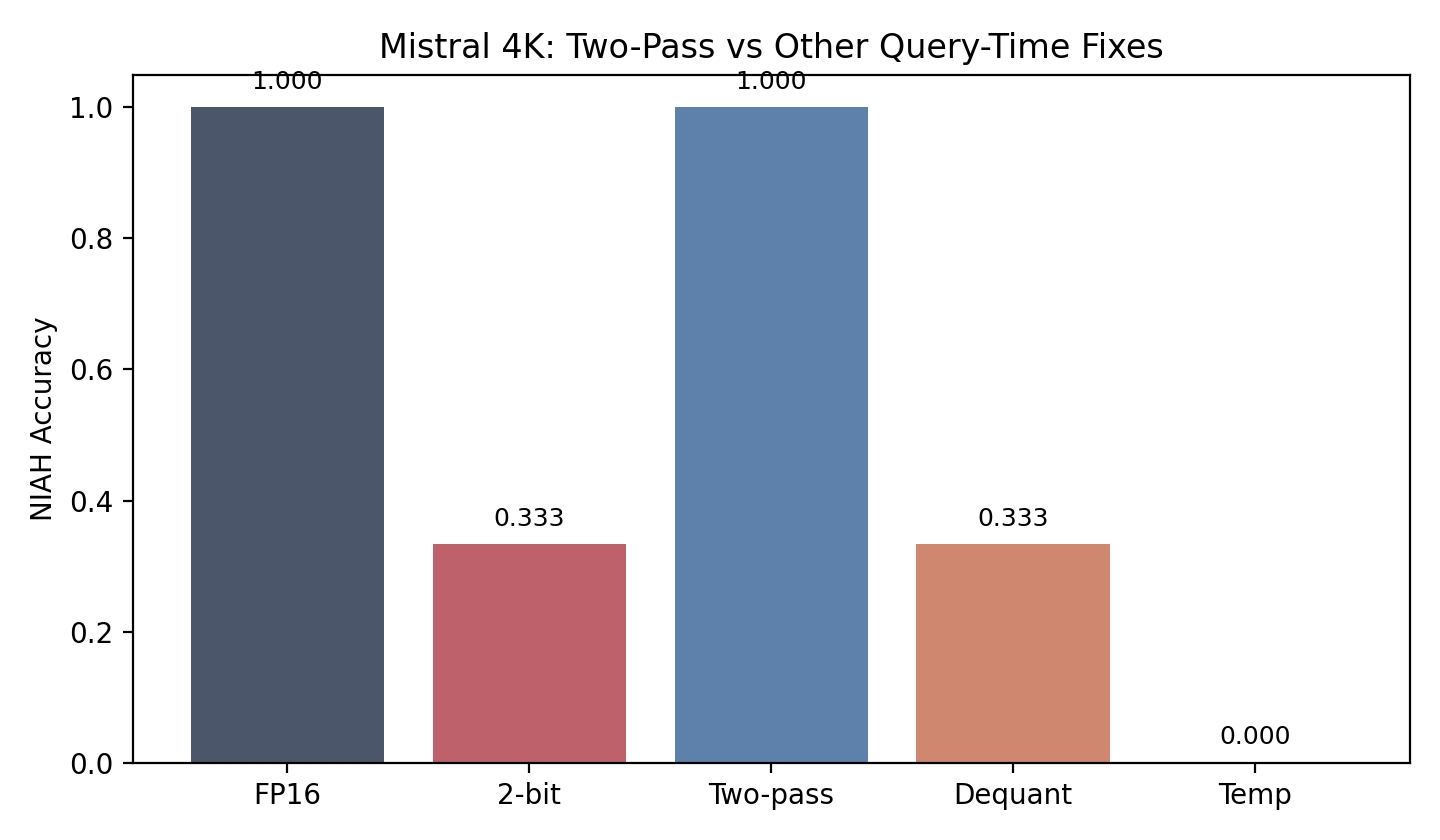
\includegraphics[width=0.9\linewidth]{../figures/selective_refine_mistral_method_compare.png}
\caption{Mistral 4K same-harness comparison. Only \texttt{two\_pass} clearly beats the bounded 2-bit baseline.}
\end{figure}

\begin{figure}[H]
\centering
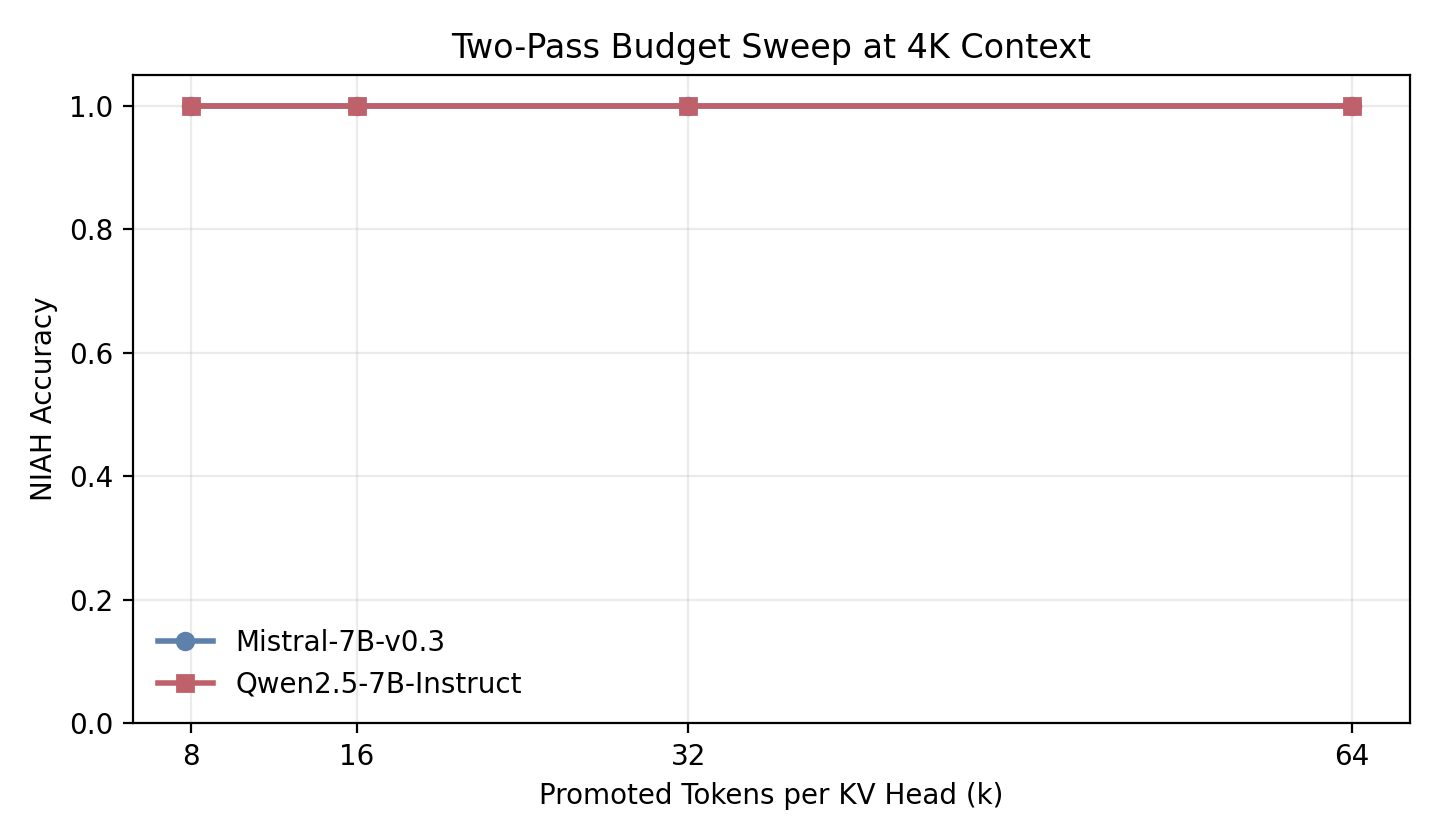
\includegraphics[width=0.9\linewidth]{../figures/selective_refine_two_pass_budget_sweep.png}
\caption{4K two-pass sweep. The grid is already saturated from \texttt{k=8}, so it shows existence of a win but not the minimum useful budget frontier.}
\end{figure}

\section{Bottom Line}

지금 상태는 top-venue method가 아니다. \texttt{two\_pass}는 좋은 diagnostic candidate이지만
먼저 reproducibility audit을 받아야 한다. QDRP는 아직 theory-level hypothesis이며,
TRIC는 현재 진단 기준으로 탈락이다. 이 wave가 다시 살아나는 유일한 길은 earlier remote win이
current code에서 재현되고, true storage-valid selective refinement를 구현했는데도 gain이 남는 경우뿐이다.

\end{document}
